\documentclass[../searching.tex]{subfiles}
\begin{document}
To search in a sorted array or string using brute force with a for loop, it takes $O(n)$ time. Binary search is designed to reduce search time if the array or string is already sorted. It uses the divide and conquer method; each time we compare our target with the middle element of the array and with the comparison result to decide the next search region: either the left half or the right half. Therefore, each step we filter out half of the array which gives the time complexity function $T(n) = T(n/2) + O(1)$, which decrease the time complexity to $O(\log n)$.

Binary Search can be applied to different tasks:
\begin{enumerate}
    \item Find Exact target, find the first position that value>= target, find the last position that value<= target.(this is called lower\_bound, and upper\_bound. 
\end{enumerate}

\subsection{Standard Binary Search and Python Module bisect}
Binary search is usually carried out on a Static sorted array or 2D matrix. There are three basic cases: (1) find the exact target that value = target; If there are duplicates, we are more likely to be asked to (2) find the first position that has value >= target; (3) find the first position that has value <= target. Here, we use two example array: one without duplicates and the other has duplicates.
\begin{lstlisting}[language=Python]
a = [2, 4, 5, 9]
b = [0, 1, 1, 1, 1, 1]
\end{lstlisting}

\paragraph{Find the Exact Target} This is the most basic application of binary search. We can set two pointers, l and r. Each time we compute the middle position, and check if it is equal to the target. If it is, return the position; if it is smaller than the target, move to the left half, otherwise, move to the right half. The Python code is given:
\begin{lstlisting}[language=Python]
def standard_binary_search(lst, target):
    l, r = 0, len(lst) - 1
    while l <= r:
        mid = l + (r - l) // 2
        if lst[mid] == target:
            return mid
        elif lst[mid] < target:
            l = mid + 1
        else:
            r = mid - 1
    return -1 # target is not found 
\end{lstlisting}
Now, run the example:
\begin{lstlisting}[language=Python]
print("standard_binary_search: ", standard_binary_search(a,3), standard_binary_search(a,4), standard_binary_search(b, 1))
\end{lstlisting}
The print out is:
\begin{lstlisting}
standard_binary_search:  -1 1 2
\end{lstlisting}
From the example, we can see that multiple \textbf{duplicates} of the target exist, it can possibly return any one of them. And for the case when the target does not exist, it simply returns -1. In reality, we might need to find a position where we can potentially insert the target to keep the sorted array sorted. There are two cases: (1) the first position that we can insert, which is the first position that has value>= target (2) and the last position we can insert, which is the first position that has value > target. For example, if we try to insert 3 in a, and 1 in b, the first position should be 1 and 1 in each array, and the last position is 1 and 6 instead.  For these two cases, we have a Python built-in Module \textbf{bisect} which offers two methods: bisect\_left() and bisect\_right() for these two cases respectively.

\paragraph{Find the First Position that value >= target} This way the target position separates the array into two halves: value < target, target\_position, value>= target. In order to meet the purpose, we make sure that if value < target, we move to the right side, else, move to the left side.
\begin{lstlisting}[language=Python]
# bisect_left, no longer need to check the mid element,
# it separate the list in to two halfs: value < target, mid,  value >= target
def bisect_left_raw(lst, target):
    l, r = 0, len(lst)-1
    while l <= r:
        mid = l + (r-l)//2
        if lst[mid] < target: # move to the right half if the value < target, till
            l = mid + 1 #[mid+1, right]
        else:# move to the left half is value >= target
            r = mid - 1  #[left, mid-1]
    return l # the final position is where
\end{lstlisting}
% Now insert the value with:
% \begin{lstlisting}[language=Python]
% lst.insert(l+1, target)
% \end{lstlisting}

\paragraph{Find the First Position that value > target} This way the target position separates the array into two halves: value <= target, target\_position, value> target. Therefore, we simply change the condition of if value < target to if value <= target, then we move to the right side.
\begin{lstlisting}[language=Python]
#bisect_right: separate the list into two halfs: value<= target, mid, value > target
def bisect_right_raw(lst, target):
    l, r = 0, len(lst)-1
    while l <= r:
        mid = l + (r-l)//2
        if lst[mid] <= target:
            l = mid + 1
        else:
            r = mid -1
    return l
\end{lstlisting}
Now, run an example:
\begin{lstlisting}[language=Python]
print("bisect left raw: find 3 in a :", bisect_left_raw(a,3), 'find 1 in b: ', bisect_left_raw(b, 1))
print("bisect right raw: find 3 in a :", bisect_right_raw(a, 3), 'find 1 in b: ', bisect_right_raw(b, 1))
\end{lstlisting}
The print out is:
\begin{lstlisting}
bisect left raw: find 3 in a : 1 find 1 in b:  1
bisect right raw: find 3 in a : 1 find 1 in b:  6
\end{lstlisting}

\paragraph{Bonus} For the last two cases, if we return the position as l-1, then we get the last position that value < target, and the last position value <= target.

\paragraph{Python Built-in Module bisect} This module provides support for maintaining a list in sorted order without having to sort the list after each insertion. It offers six methods as shown in Table~\ref{tab:method_bisect}. However, only two are most commonly used: bisect\_left and bisect\_right.
\begin{table}[h]
\begin{small}
\centering
\noindent\captionof{table}{ Methods of \textbf{bisect}}
 \noindent \begin{tabular}{|p{0.25\columnwidth}|p{0.75\columnwidth}| }
  \hline
Method & Description   \\ \hline
bisect\_left(a, x, lo=0, hi=len(a)  &  The parameters lo and hi may be used to specify a subset of the list; the function is the same as bisect\_left\_raw  \\\hline
bisect\_right(a, x, lo=0, hi=len(a)  &  The parameters lo and hi may be used to specify a subset of the list; the function is the same as bisect\_right\_raw  \\\hline
bisect(a, x, lo=0, hi=len(a))  &Similar to bisect\_left(), but returns an insertion point which comes after (to the right of) any existing entries of x in a.\\ \hline
insort\_left(a, x, lo=0, hi=len(a))  &This is equivalent to a.insert(bisect.bisect\_left(a, x, lo, hi), x).\\ \hline
insort\_right(a, x, lo=0, hi=len(a)) & This is equivalent to a.insert(bisect.bisect\_right(a, x, lo, hi), x).\\ \hline
insort(a, x, lo=0, hi=len(a)) & Similar to insort\_left(), but inserting x in a after any existing entries of x.\\ \hline
\end{tabular}
  \label{tab:method_bisect}
  \end{small}
\end{table} 
Let's see come examplary code:
\begin{lstlisting}[language=Python]
from bisect import bisect_left,bisect_right, bisect
print("bisect left: find 3 in a :", bisect_left(a,3), 'find 1 in b: ', bisect_left(b, 1)) # lower_bound, the first position that value>= target
print("bisect right: find 3 in a :", bisect_right(a, 3), 'find 1 in b: ', bisect_right(b, 1)) # upper_bound, the last position that value <= target
\end{lstlisting}
The print out is:
\begin{lstlisting}
bisect left: find 3 in a : 1 find 1 in b:  1
bisect right: find 3 in a : 1 find 1 in b:  6
\end{lstlisting}
\subsection{Binary Search in Rotated Sorted Array}
\label{concept_binary_search_in_array}
The extension of the standard binary search is on array that the array is ordered in its own way like rotated array. 

\paragraph{Binary Search in Rotated Sorted Array } (See LeetCode problem, 33. Search in Rotated Sorted Array (medium). Suppose an array (without duplicates) sorted in ascending order is rotated at some pivot unknown to you beforehand. (i.e., 0 1 2 4 5 6 7 might become 4 5 6 7 0 1 2). You are given a target value to search. If found in the array return its index, otherwise return -1. You may assume no duplicate exists in the array.
\begin{lstlisting}[numbers=none]
Example 1:

Input: nums = [3, 4,5,6,7,0,1,2], target = 0
Output: 5

Example 2:

Input: nums = [4,5,6,7,0,1,2], target = 3
Output: -1
\end{lstlisting}

In the rotated sorted array, the array is not purely monotonic. Instead, there is one drop in the array because of the rotation, where it cuts the array into two parts. Suppose we are starting with a standard binary search with example 1, at first, we will check index 3, then we need to move to the right side?  Assuming we compare our middle item with the left item, 
\begin{lstlisting}[numbers=none]
if nums[mid] > nums[l]: # the left half is sorted
elif nums[mid] < nums[l]: # the right half is sorted
else: # for case like [1,3], move to the right half
\end{lstlisting}
For a standard binary search, we simply need to compare the target with the middle item to decide which way to go. In this case, we can use objection. Check which side is sorted, because no matter where the left, right and the middle index is, there is always one side that is sorted. So if the left side is sorted, and the value is in the range of the [left, mid], then we move to the left part, else we object the left side, and move to the right side instead. 
\begin{figure}[h]
    \centering
    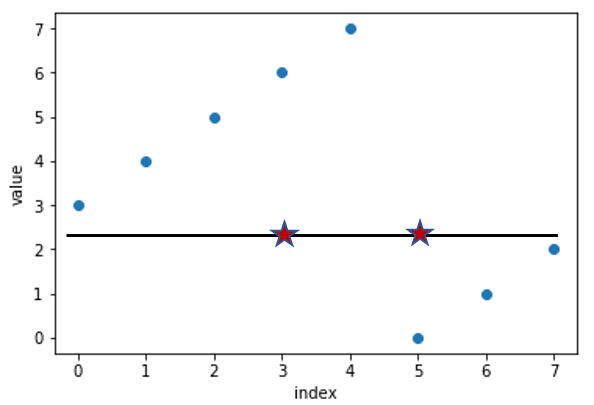
\includegraphics[width=0.7\columnwidth]{fig/rotated_array.png}
    \caption{Example of Rotated Sorted Array}
    \label{fig:rotated_sorted_array}
\end{figure}

The code is shown:
\begin{lstlisting}[language=Python]
'''implemente the rotated binary search'''
def RotatedBinarySearch(nums, target):
    if not nums:
        return -1
   
    l,r = 0,len(nums)-1
    while l<=r:
        mid = l+ (r-l)//2
        if nums[mid] == target:
            return mid
         if nums[l] < nums[mid]: # if the left part is sorted
                if nums[l] <= target <= nums[mid]:
                    r = mid-1
                else:
                    l = mid+1
            elif nums[l] > nums[mid]: # if the right side is sorted
                if nums[mid] <= target <= nums[r]:
                    l = mid+1
                else:
                    r = mid-1
            else:
                l = mid + 1
    return -1
\end{lstlisting}
\begin{bclogo}[couleur = blue!30, arrondi=0.1,logo=\bccrayon,ombre=true]{What happens if there is duplicates in the rotated sorted array? } In fact, similar comparing rule applies: 
\begin{lstlisting}[numbers=none]
if nums[mid] > nums[l]: # the left half is sorted
elif nums[mid] < nums[l]: # the right half is sorted
else: # for case like [1,3], or [1, 3, 1, 1, 1] or [3, 1, 2, 3, 3, 3]
   only l++
\end{lstlisting}
\end{bclogo}




%%%%%%%%%%%%%%binary search on result space%%%%%%%
\subsection{Binary Search on Result Space}
If the question gives us the context: the target is in the range [left, right], we need to search the first or last position that satisfy a condition function. We can apply the concept of standard binary search and bisect\_left and bisect\_right and its mutant. Where we use the condition function to replace the value comparison between target and element at middle position. The steps we need:
\begin{enumerate}
    \item get the result search range [l, r] which is the initial value for l and r pointers. 
    \item decide the valid function to replace such as if lst[mid] < target 
    \item decide which binary search we use: standard, bisect\_left/ bisect\_right or its mutant.
\end{enumerate}

For example: 
\begin{examples}[resume]
\item \textbf{441. Arranging Coins (easy)}. You have a total of n coins that you want to form in a staircase shape, where every k-th row must have exactly k coins. Given n, find the total number of full staircase rows that can be formed. n is a non-negative integer and fits within the range of a 32-bit signed integer.
\begin{lstlisting}[numbers=none]
Example 1:

n = 5

The coins can form the following rows:
*
* *
* *

Because the 3rd row is incomplete, we return 2.
\end{lstlisting}

\textbf{Analysis: } Given a number n>=1, the minimum row is 1, and the maximum is n. Therefore, our possible result range is [1, n]. These can be treated as indexes of the sorted array. For a given row, we write a function to check if it is possible. We need a function $r* (r+1) // 2 <= n$. For this problem, we need to search in the range of [1, n] to find the last position that is valid. This is bisect\_left or bisect\_right, where we use the function replace the condition check:
\begin{lstlisting}[language=Python]
def arrangeCoins(self, n):
    def isValid(row):
        return (row*(row+1))//2 <= n
    # we need to find the last position that is valid (<=)
    def bisect_right():
        l, r = 1, n
        while l <= r:
            mid = l + (r-l) // 2
            if isValid(mid): # replaced compared with the standard binary search
                l = mid + 1
            else:
                r = mid - 1
        return l-1
    return bisect_right()
\end{lstlisting}
\item \textbf{278. First Bad Version.} You are a product manager and currently leading a team to develop a new product. Unfortunately, the latest version of your product fails the quality check. Since each version is developed based on the previous version, all the versions after a bad version are also bad.

Suppose you have n versions [1, 2, ..., n] and you want to find out the first bad one, which causes all the following ones to be bad.

You are given an API bool isBadVersion(version) which will return whether version is bad. Implement a function to find the first bad version. You should minimize the number of calls to the API.

Solution: we keep doing binary search until we have searched all possible areas.
\begin{lstlisting}[language = Python]
class Solution(object):
    def firstBadVersion(self, n):
        """
        :type n: int
        :rtype: int
        """
        l,r=0,n-1
        last = -1
        while l<=r:
            mid = l+(r-l)//2
            if isBadVersion(mid+1): #move to the left, mid is index, s
                r=mid-1
                last = mid+1 #to track the last bad one
            else:
                l=mid-1
        return last
\end{lstlisting}
\end{examples}
% \subsection{Bisection Method} (second edition)
% The binary search principle can be used to find the root of a function that may be difficult to compute mathematically. We have not seen any problems that require this method on LeetCode yet. Thus we define the problem as:

% Find the monthly payment for a loan: You want to buy a car using loan and want to pay in monthly installment of d d
% \subsection{Python Library}
% Python has \textbf{bisect} module for binary search. 
% \begin{lstlisting}[numbers=none]
% bisect.bisect_left(a,    x):  Return the leftmost index where we can  insert x into a to maintain sorted order! Leftmost rl that satisfy: x<=a[rl]

% bisect.bisect_right(a,    x):  Return the rightmost index where we can  insert x into a to maintain sorted order! Right most rr that satisfy: x>=a[rr]
% \end{lstlisting}
% For example:
% \begin{lstlisting}[language=Python]
% from bisect import bisect_left,bisect_right
% a = [1,    2,    3,    3,    3,    4,    5]
% p1, p2= bisect_left(a,3), bisect_right(a, 3)
% print(p1, p2)
% # output
% # 2, 5
% \end{lstlisting}

\subsection{LeetCode Problems}
\begin{examples}
\item \textbf{35. Search Insert Position (easy).} Given a sorted array and a target value, return the index if the target is found. If not, return the index where it would be if it were inserted in order.

You can assume that there are no duplicates in the array.
\begin{lstlisting}[numbers=none]
Example 1:

Input: [1,3,5,6], 5
Output: 2

Example 2:
Input: [1,3,5,6], 2
Output: 1

Example 3:
Input: [1,3,5,6], 7
Output: 4

Example 4:
Input: [1,3,5,6], 0
Output: 0
\end{lstlisting}

\textbf{Solution: Standard Binary Search Implementation.} For this problem, we just standardize the Python code of binary search, which takes $O(logn)$ time complexity and O(1) space complexity without using recursion function. In the following code, we use exclusive right index with len(nums), therefore it stops if l == r; it can be as small as 0 or as large as n of the array length for numbers that are either smaller or equal to the nums[0] or larger or equal to nums[-1]. We can also make the right index inclusive. 
\begin{lstlisting}[language = Python]
# exclusive version
def searchInsert(self, nums, target):
    l, r = 0, len(nums) #start from 0, end to the len (exclusive)
    while l < r:
        mid = (l+r)//2
        if nums[mid] < target: #move to the right side
            l = mid+1
        elif nums[mid] > target: #move to the left side, not mid-1
             r= mid
        else: #found the traget
            return mid
    #where the position should go
    return l
\end{lstlisting}

\begin{lstlisting}[language = Python]
# inclusive version
def searchInsert(self, nums, target):
   l = 0
    r = len(nums)-1
    while l <= r:
        m = (l+r)//2
        if target > nums[m]: #search the right half
            l = m+1
        elif target < nums[m]: # search for the left half
            r = m-1
        else:
            return m
    return l
\end{lstlisting}
\end{examples}
Standard binary search
\begin{enumerate}
    \item 611. Valid Triangle Number (medium)
    \item 704. Binary Search (easy)
    
\item  74. Search a 2D Matrix) Write an efficient algorithm that searches for a value in an m x n matrix. This matrix has the following properties:
\begin{enumerate}
    \item Integers in each row are sorted from left to right.
    \item The first integer of each row is greater than the last integer of the previous row.
    \end{enumerate}
\begin{lstlisting}[numbers=none]
For example,
Consider the following matrix:

[
  [1,   3,  5,  7],
  [10, 11, 16, 20],
  [23, 30, 34, 50]
]

Given target = 3, return true.
\end{lstlisting}

Solution: 2D matrix search, time complexity from $O(n^2)$ to $O(lgm+lgn)$.
\begin{lstlisting}[language = Python]
def searchMatrix(self, matrix, target):
        """
        :type matrix: List[List[int]]
        :type target: int
        :rtype: bool
        """
        
        if not matrix:
            return False
        row, col = len(matrix), len(matrix[0])
        if row==0 or col==0: #for [[]]
            return False
        sr, er = 0, row-1
        #fisrst search the mid row
        while sr<=er:
            mid = sr+(er-sr)//2
            if target>matrix[mid][-1]: #go to the right side
                sr=mid+1
            elif target < matrix[mid][0]: #go the the left side
                er = mid-1
            else: #value might be in this row
                #search in this row
                lc, rc = 0, col-1
                while lc<=rc:
                    midc = lc+(rc-lc)//2
                    if matrix[mid][midc]==target:
                        return True
                    elif target<matrix[mid][midc]: #go to left
                        rc=midc-1
                    else:
                        lc=midc+1
                return False
        return False
\end{lstlisting}

Also, we can treat is as one dimensional, and the time complexity is $O(lg(m*n))$, which is the same as $O(log(m)+log(n))$.
\begin{lstlisting}[language = Python]
class Solution:
    def searchMatrix(self, matrix, target):
        if not matrix or target is None:
            return False

        rows, cols = len(matrix), len(matrix[0])
        low, high = 0, rows * cols - 1
        
        while low <= high:
            mid = (low + high) / 2
            num = matrix[mid / cols][mid % cols]

            if num == target:
                return True
            elif num < target:
                low = mid + 1
            else:
                high = mid - 1
        
        return False
\end{lstlisting}
\end{enumerate}

Check \url{http://www.cnblogs.com/grandyang/p/6854825.html} to get more examples.

Search on rotated and 2d matrix:
\begin{enumerate}
    \item 81. Search in Rotated Sorted Array II (medium) 
    \item 153. Find Minimum in Rotated Sorted Array (medium) The key here is to compare the mid with left side, if mid-1 has a larger value, then that is the minimum 
    \item 154. Find Minimum in Rotated Sorted Array II (hard)
\end{enumerate}
Search on Result Space:
\begin{enumerate}
    \item 367. Valid Perfect Square (easy) (standard search)
    \item 363. Max Sum of Rectangle No Larger Than K (hard)
    \item 354. Russian Doll Envelopes (hard)
    \item 69. Sqrt(x) (easy)
\end{enumerate}
\end{document}